\documentclass{article}
\usepackage{graphicx}
\usepackage{nopageno}
\usepackage{txfonts}
\usepackage[usenames]{color}
%\usepackage[T2A]{fontenc}
\usepackage[utf8]{inputenc}
\usepackage{subcaption}
\usepackage{caption}


\begin{document}
\begin{center}
	\begin{figure}[htbp] %  figure placement: here, top, bottom, or page
		\begin{subfigure}[b]{0.6\textwidth}
		   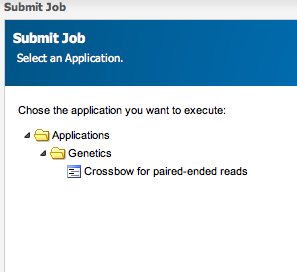
\includegraphics[width=\textwidth]{a.png} 
		\subcaption{Cloudgene: selecting a job to run}
		\end{subfigure}
		\begin{subfigure}[b]{0.6\textwidth}
		   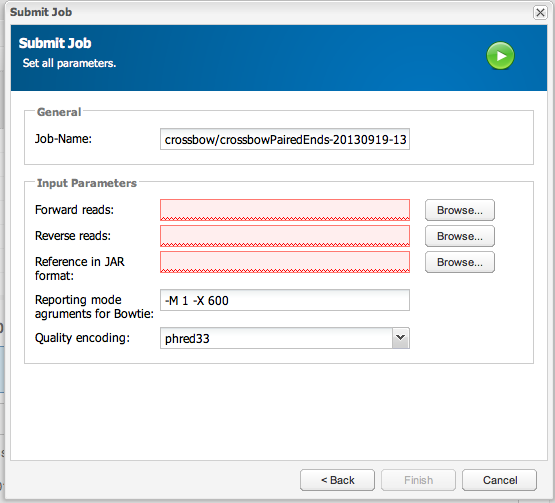
\includegraphics[width=\textwidth]{b.png} 
			\subcaption{Cloudgene: specifying job parameters}
		\end{subfigure}
		\caption{An example of a job setup with the Cloudgene, a web-based GUI wrapper, providing a smooth user experience even for novice users.}
		\label{fig:fig5}
	\end{figure}
\end{center}
\end{document}
